\documentclass[11pt,letterpaper]{report}
\usepackage{amssymb,amsfonts,color,graphicx,amsmath,enumerate}
\usepackage{tikz}
\usepackage{amsthm}
\usepackage{bbm}
\usepackage{hyperref}

\newcommand{\naturals}{\mathbb{N}}
\newcommand{\integers}{\mathbb{Z}}
\newcommand{\complex}{\mathbb{C}}
\newcommand{\reals}{\mathbb{R}}
\newcommand{\mcal}[1]{\mathcal{#1}}
\newcommand{\rationals}{\mathbb{Q}}
\newcommand{\Lp}[2]{\left\|{#1}\right\|_{L^{#2}}}
\newcommand{\field}{\mathbb{F}}
\newcommand{\affine}{\mathbb{A}}
\newcommand{\E}{\mathbb{E}}
\newcommand{\Prob}{\mathbb{P}}
\newcommand{\Var}{\text{Var}}
\newcommand{\ind}{\mathbbm{1}}
\newcommand{\Cov}{\text{Cov}}

\newenvironment{solution}
{\begin{proof}[Solution]}
{\end{proof}}

\voffset=-3cm
\hoffset=-2.25cm
\textheight=24cm
\textwidth=17.25cm
\addtolength{\jot}{8pt}
\linespread{1.3}

\begin{document}
\begin{center}
{\bf \Large Math 175 - Homework 7}
\vspace{0.2cm}
\hrule
\end{center}

\begin{enumerate}
	\item Let $G$ be bipartite graph with parts $X$ and $Y$.
	\begin{enumerate}
		\item Show that $\sum_{v\in X}d(v) = \sum_{v\in Y}d(v)$.
		\item Deduce that if $G$ is $k$-regular (every vertex has degree $k$) with $k\geq 1$, then $|X| = |Y|$.
	\end{enumerate}

	\vfill

	\item Let $G$ be the graph whose vertex set is the set of $k$-tuples with coordinates in $\{0, 1\}$, with $x$ adjacent to $y$ when $x$ and $y$ differ in exactly one position. Determine whether $G$ is bipartite.
	\vfill

	\item An \textit{isomorphism} between simple graphs $G$ and $H$ is a bijection $f: V(G)\to V(H)$ that preserves adjacency (that is, the vertices $u$ and $v$ are adjacent in $G$ if and only if their images $f(u)$ and $f(v)$ are adjacent in $H$).
	\begin{enumerate}
		\item Are the graphs $G$ and $H$ shown below isomorphic? If so, give an isomorphism. If not, explain why not.
		\begin{figure}[h]
			\center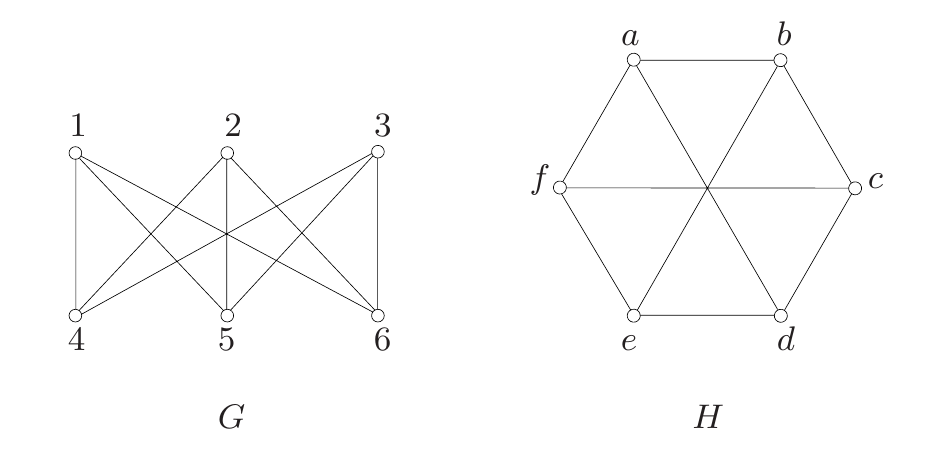
\includegraphics[scale=0.5]{iso.png}
		\end{figure}
		\item If two graphs have the same number of vertices and edges, are they necessarily isomorphic? If so, prove it. If not, give a counterexample.
		\item Show that any isomorphism between two graphs maps each vertex to a vertex of the same degree.
		\item Let $G$ be a connected graph. Show that every graph which is isomorphic to $G$ is connected.
	\end{enumerate}
	\vfill\pagebreak


	\item A \textit{triangle-free} graph is one which contains no triangles. Let $G$ be a simple $n$-vertex, $m$-edge, triangle-free graph.
	\begin{enumerate}
		\item Show that $d(x) + d(y) \leq n$ for all adjacent $x$ and $y$.
		\item Deduce that $\sum_{v\in V}d(v)^2 \leq mn$.
		\item Apply the Cauchy-Schwarz inequality to deduce that $m\leq n^2/4$. Recall the Cauchy-Schwarz inequality says that
		\[
		\left(\sum_{i=1}^n a_ib_i\right)^2\leq \sum_{i=1}^na_i^2\cdot \sum_{i=1}^nb_i^2.
		\]
		\item For each positive integer $n$, show that this bound can be realized. That is, find a simple triangle-free graph $G$ with $m = \lfloor n^2/4\rfloor$.
	\end{enumerate}
	\vfill
\end{enumerate}


\end{document}